In this report, the general use of drones indoor will be examined. There have been much development of drones for outdoor use, but the indoor use of drones have not been developed as much, most because safety precautions have to be taken.
Some of these precautions will be examined and solved through this report. The goal with this report is to make it possible to fly a drone indoor safely. \newline
However, today drones are mainly used for outdoor flying, both long distance and short distance flying. Each drone type has different purposes depending on how the drone is designed.
\newline
To make it possible to fly an off-the-shelf drone indoor, a few precautions is needed. 
%%%%%%%%%%%%%%%%%%%%%%%%%%%%%%%
One of the precautions there needs to be taken, when flying a drone indoor, is to secure that it does not bump into objects, like a wall. This can be done by making an area around the drone as a virtual bubble, that will detect objects, as the figure \ref{fig:introSaftyBobble} is illustrating. %As seen on figure \ref{fig:introSaftyBobble} the focus for this project will be to implement this solution for a quadcopter.
\begin{figure}[H]
    \centering
    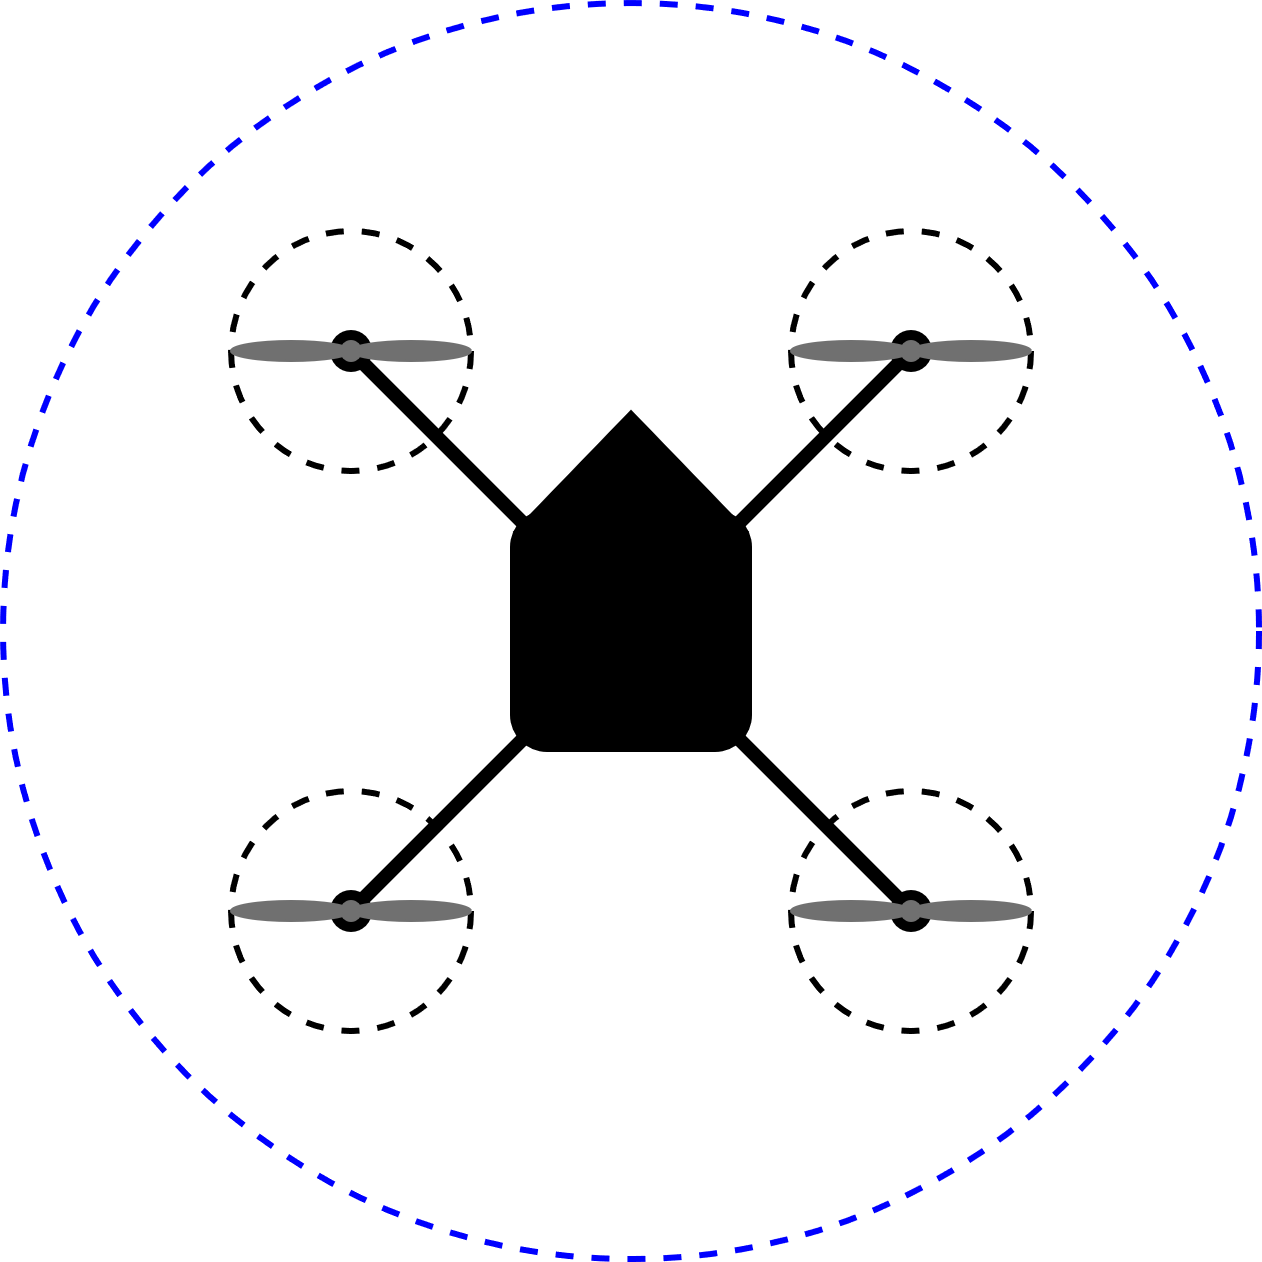
\includegraphics[width=0.35\textwidth]{figures/ch_intro/BobleOmDrone.png}
    \caption{illustration of a "safety bubble" around a drone.}
    \label{fig:introSaftyBobble}
\end{figure}
%%%%%%%%%%%%%%%%%%%%%%%%%%%%%%%





\section{Drones}\label{s:drones}
To start out this report, two questions should be resolved, what is a drone and what is it used for. 
A drone is also called a UAV, which is short for unmanned aerial vehicles. A drone can be controlled in different ways, by either software or remote controller. Drones are not exclusively unmanned flying vehicles, but can also be a driving vehicle. Drones is the definition of unmanned vehicles, in this report the word drones will be used for flying drones.   
A drone has mainly two ways it is designed, fixed wing and multirotor \cite{drones_type}. The two types can be seen in figure \ref{fig:drones_type}. To learn more about these two types, some of the applications for each of the types will be reviewed in the next section.

\begin{figure}[h]
\centering
    \begin{subfigure}[h]{0.45\textwidth}
        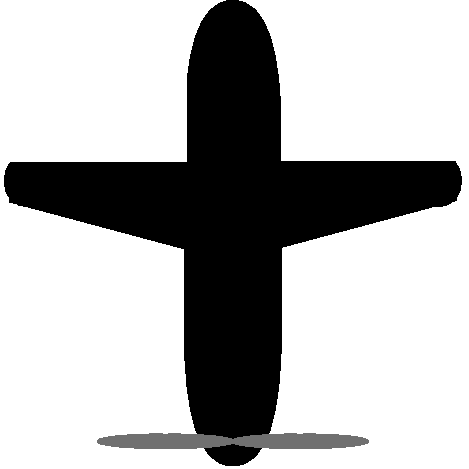
\includegraphics[width=\textwidth]{figures/PA/Fixedwing.pdf}
        \caption{Example of a fixed wing drone}
        \label{fig:fixedwing}
    \end{subfigure}
    ~
    \begin{subfigure}[h]{0.45\textwidth}
        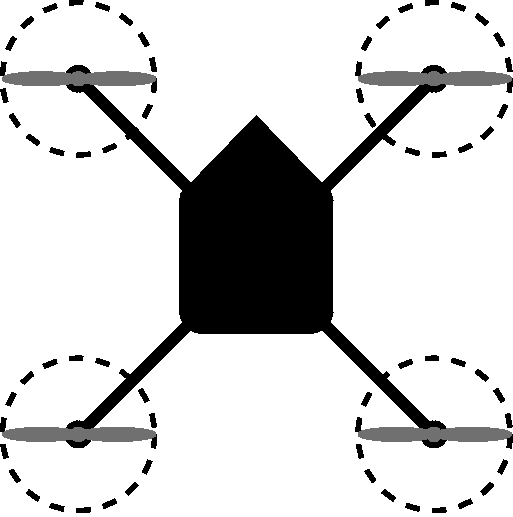
\includegraphics[width=\textwidth]{figures/PA/Quadcopter.pdf}
        \caption{Example of a multirotor drone}
        \label{fig:multirotor}
    \end{subfigure}
    \caption{Two types of drones}
    \label{fig:drones_type}
\end{figure}

 

%https://www.businessinsider.com/commercial-drone-uses-agriculture-business-military-2017-8?r=US&IR=T&IR=T
%\section{Drone applications}
%The use of drone in the industry and business has evolved a lot in the last few years, and the use evolves more each year. 
%The industries where drones are mostly used today are farming and military.
%\newline
%The use of drones in farming has evolved the traditional way of farming, as the drone can do things the farmer cannot do himself. The drones most used drone for farming, is multirotor drones. The drones can scan whole fields in minutes, and obtain knowledge of the crop's health. 
%\newline
%\newline
%The military has used drones since 1955, mainly for things where it is too dangerous for soldiers. This includes both combat missions and supervision. The military mostly use fixed wing drones because they are bigger and can carry a bigger cargo. They also have a much longer fly time. The fixed wing drone comes in all sizes, from small hand launched drones to large planes.
%\newline
%\newline
%It is not only in the farming industry and military drones have been used, or are being used.
%Drones is also being used for delivery of food and medicine to places where humans cannot get to. Such as areas where natural disasters have appeared, where the drones can give air support to the area \cite{drones_in_generel}.
%\newline
%In the future drones would be used to a lot more things, for example the multirotor drone will be used for exploration of mines and crash sites. Thus drones have to work in small and  narrow places, where they always have to know if it can fit. The multirotor drone will be used for this because it has a better mobility, than a fixed wing drone which needs a bigger space to fly. 









